\documentclass[tikz,border=2pt]{standalone}
\usepackage{pgfplots}
\pgfplotsset{compat=1.18}
\usepgfplotslibrary{groupplots}
\usetikzlibrary{arrows.meta}

\begin{document}
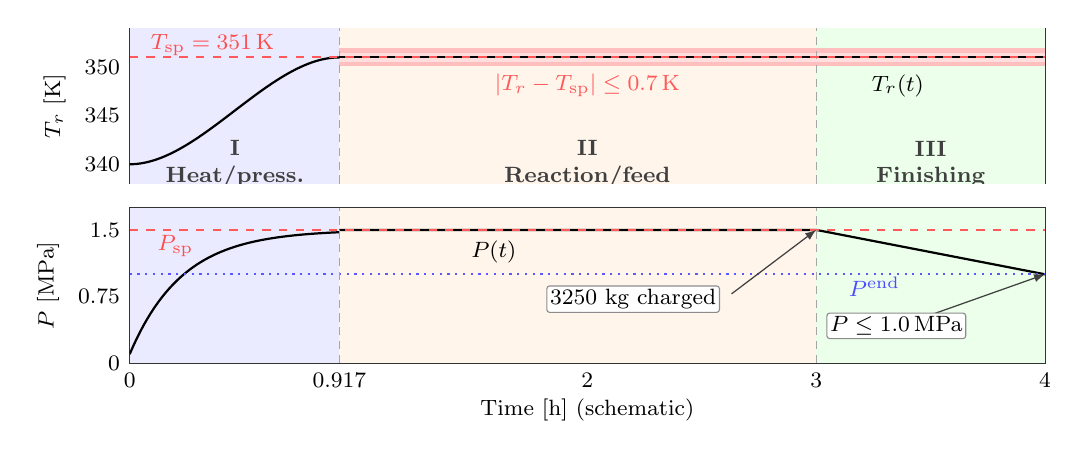
\begin{tikzpicture}
\pgfplotsset{
  every axis/.append style={
    width=5.2in,
    height=1.40in,
    xmin=0,
    xmax=4,
    xtick={0,0.916667,2,3,4},
    xticklabels={0,0.917,2,3,4},
    axis line style={black!80},
    tick style={black!80},
    tick label style={font=\footnotesize},
    label style={font=\footnotesize},
    grid=both,
    major grid style={black!22,dotted},
    minor grid style={black!10,dotted},
  }
}

\begin{groupplot}[
  group style={
    group size=1 by 2,
    vertical sep=0.12in
  }
]

\nextgroupplot[
  ymin=338,
  ymax=354,
  ytick={340,345,350},
  ylabel={$T_r$ [K]},
  xticklabels=\empty,
]
\path[fill=blue!8] (axis cs:0,338) rectangle (axis cs:0.916667,354);
\path[fill=orange!8] (axis cs:0.916667,338) rectangle (axis cs:3,354);
\path[fill=green!8] (axis cs:3,338) rectangle (axis cs:4,354);
\path[fill=red!13] (axis cs:0.916667,350.3) rectangle (axis cs:4,351.7);
\addplot[red!25,line width=1.6pt] coordinates {(0.916667,350.3) (4,350.3)};
\addplot[red!25,line width=1.6pt] coordinates {(0.916667,351.7) (4,351.7)};
\addplot[black!35,densely dashed] coordinates {(0.916667,338) (0.916667,354)};
\addplot[black!35,densely dashed] coordinates {(3,338) (3,354)};
\addplot[black,thick,domain=0:0.916667,samples=60] {340 + 11*(3*(x/0.916667)^2-2*(x/0.916667)^3)};
\addplot[black,thick] coordinates {(0.916667,351.0) (4,351.0)};
\addplot[red!65,thick,dashed] coordinates {(0,351.0) (4,351.0)};
\node[font=\footnotesize\bfseries,align=center,text=black!75] at (axis cs:0.46,340.0) {I\\Heat/press.};
\node[font=\footnotesize\bfseries,align=center,text=black!75] at (axis cs:2.00,340.0) {II\\Reaction/feed};
\node[font=\footnotesize\bfseries,align=center,text=black!75] at (axis cs:3.50,340.0) {III\\Finishing};
\node[font=\footnotesize,anchor=west,text=red!70] at (axis cs:0.05,352.3) {$T_{\mathrm{sp}}=351\,\mathrm{K}$};
\node[font=\footnotesize,text=red!65] at (axis cs:2.00,348.1) {$|T_r-T_{\mathrm{sp}}|\le0.7\,\mathrm{K}$};
\node[font=\footnotesize,anchor=west] at (axis cs:3.20,348.1) {$T_r(t)$};

\nextgroupplot[
  ymin=0,
  ymax=1.75,
  ytick={0,0.75,1.5},
  ylabel={$P$ [MPa]},
  xlabel={Time [h] (schematic)},
  xlabel style={yshift=0.6ex},
]
\path[fill=blue!8] (axis cs:0,0) rectangle (axis cs:0.916667,1.75);
\path[fill=orange!8] (axis cs:0.916667,0) rectangle (axis cs:3,1.75);
\path[fill=green!8] (axis cs:3,0) rectangle (axis cs:4,1.75);
\addplot[black,thick,domain=0:0.916667,samples=60] {1.5 - 1.4*exp(-x/0.23)};
\addplot[black,thick] coordinates {(0.916667,1.5) (3,1.5) (4,1.0)};
\addplot[red!65,thick,dashed] coordinates {(0,1.5) (4,1.5)};
\addplot[blue!65,thick,dotted] coordinates {(0,1.0) (4,1.0)};
\addplot[black!35,densely dashed] coordinates {(0.916667,0) (0.916667,1.75)};
\addplot[black!35,densely dashed] coordinates {(3,0) (3,1.75)};
\node[font=\footnotesize,anchor=west,text=red!70] at (axis cs:0.08,1.32) {$P_{\mathrm{sp}}$};
\node[font=\footnotesize,anchor=west,text=blue!70] at (axis cs:3.10,0.86) {$P^{\mathrm{end}}$};
\node[font=\footnotesize,anchor=west] at (axis cs:1.45,1.25) {$P(t)$};
\draw[-{Latex[length=1.4mm]},black!75,line width=0.45pt]
  (axis cs:2.63,0.78) -- (axis cs:3.0,1.5);
\node[font=\footnotesize,fill=white,draw=black!45,rounded corners=1pt,inner sep=1.2pt]
  at (axis cs:2.20,0.72) {3250 kg charged};
\draw[-{Latex[length=1.4mm]},black!75,line width=0.45pt]
  (axis cs:3.42,0.47) -- (axis cs:4.0,1.0);
\node[font=\footnotesize,fill=white,draw=black!45,rounded corners=1pt,inner sep=1.2pt]
  at (axis cs:3.35,0.42) {$P\le1.0\,\mathrm{MPa}$};

\end{groupplot}
\end{tikzpicture}
\end{document}
